\documentclass[11pt,letterpaper,reqno]{amsart}
\usepackage{tikz}
\usetikzlibrary{positioning,shapes.geometric,arrows.meta}
\usepackage{amssymb,amsmath,amsthm,amsfonts}
\usepackage{bbm}
\usepackage{enumitem}
\usepackage{pgfplots}
\pgfplotsset{compat=1.18}
\usepackage{booktabs,graphicx}
\usepackage[T1]{fontenc}
\usepackage{doi,float}
\usepackage[expansion=false]{microtype}
\addtolength{\hoffset}{-1.5cm}\addtolength{\textwidth}{3cm}
\addtolength{\voffset}{-1cm}\addtolength{\textheight}{2cm}
\usepackage{bookmark}
\usepackage{hyperref}
\hypersetup{pdfstartview={FitH},hidelinks,hypertexnames=false,
  pdftitle={The quadratic Tang--Zhang inequality for critical points of polynomials},
  pdfauthor={Teng Zhang}}
\newtheorem{thm}{Theorem}[section]
\newtheorem{lem}[thm]{Lemma}
\newtheorem{prop}[thm]{Proposition}
\newtheorem{cor}[thm]{Corollary}
\newtheorem{claim}{Claim}
\newtheorem{prob}[thm]{Problem}
\newtheorem{ques}[thm]{Question}
\newtheorem{conj}[thm]{Conjecture}
\theoremstyle{definition}
\newtheorem{eg}[thm]{Example}
\newtheorem{rem}[thm]{Remark}
\newtheorem{defin}[thm]{Definition}
\numberwithin{equation}{section}
\newcommand{\D}{\overline{\mathbb D}}
\newcommand{\dd}{\,\mathrm d}
\newcommand{\e}{\mathrm e}
\newcommand{\Ree}{\operatorname{Re}}
\newcommand{\M}{\mathcal M}
\newcommand{\code}[1]{\texttt{\detokenize{#1}}}
\makeatother

\begin{document}
\title[The quadratic Tang--Zhang inequality]
{The quadratic Tang--Zhang inequality for critical points of polynomials}
\author[T.~Zhang]{Teng Zhang}
\address{School of Mathematics and Statistics, Xi'an Jiaotong University, Xi'an 710049, P. R. China}
\email{teng.zhang@stu.xjtu.edu.cn}
\subjclass[2020]{Primary 30C10; Secondary 26D10, 30C15}
\keywords{Sendov's conjecture; polynomial zeros; critical points; inequalities; computer-assisted proof}
\date{September 15, 2026}
\begin{abstract}
Let $p$ be a polynomial of degree $n\ge2$ whose zeros lie in the closed unit disk, and let $c_1,\ldots,c_{n-1}$ be its critical points, counted with multiplicity. We prove that
$\sum_{j=1}^{n-1}|\zeta-c_j|^{-2}\ge n-1$
at every zero $\zeta$ of $p$. Equality holds precisely when $p$ is a nonzero constant multiple of $z^n-\omega$, where $|\omega|=1$. The corresponding inequality holds for every exponent $\lambda\ge2$, with the same equality cases.
\end{abstract}
\maketitle
\enlargethispage{2pt}

\section{Introduction}\label{sec:intro}

The Gauss--Lucas theorem locates the critical points of a polynomial in the convex hull of its zeros. It does not, by itself, explain how close a critical point must be to a prescribed zero. In 1958 Sendov proposed that, when all the zeros lie in the closed unit disk, every zero has a critical point within distance one. His account of the origin of the problem appears in \cite[pp.~284--285]{Sen02}. The conjecture entered Hayman's collection as Problem~4.5 under the name of Ilieff \cite{Hay67}; the attribution and the circumstances of its transmission are explained in \cite[p.~285]{Sen02}.

The boundary case was established by Rubinstein \cite[pp.~159--160, Theorem~1]{Rub68}, including the exceptional configuration $z^n-1$. Meir and Sharma proved the conjecture for quintics \cite[pp.~466--467, Theorem~4]{MS69}, and Brown and Xiang eventually covered all degrees at most eight \cite[Abstract]{BX99}. A different line of work concerned large degrees and zeros near the boundary. Bojanov, Rahman, and Szynal obtained a radius tending to one with the degree \cite{BRS85}; see also the precise formulation in \cite[pp.~287--288, (3)]{Sen02}. Near-boundary results were proved independently by Miller \cite{Mil93} and V\^aj\^aitu and Zaharescu \cite{VZ93}, and made quantitative by Chijiwa \cite{Chi11}. D\'egot established a high-degree result with the distinguished zero fixed in $(0,1)$ \cite[author version, p.~7, Theorem~9]{Deg14}; Chalebgwa obtained an explicit bound in that setting \cite[author version, p.~1, Theorem~1.1]{Cha20}. Tao subsequently proved Sendov's conjecture for all sufficiently large degrees \cite[author version, p.~2, Theorem~1.2]{Tao22}. The introduction to \cite[arXiv version, pp.~3--5]{Tao22} explains how these results address different ranges of the distinguished zero.

More recently, Mazur released a computer-assisted proof of Sendov's conjecture together with exact certificates and a separate Lean development \cite[pp.~1--2, Theorem~1.1]{Maz26}. Tao's subsequent exposition isolates the polynomial identities behind that argument and discusses its strict form \cite[Sections~1--4]{Tao26}. The present paper uses those identities, but addresses a different obstruction. A proof of Sendov's conjecture excludes configurations in which \emph{every} reciprocal critical-point distance is less than one. The inequality considered here requires excluding configurations in which only their \emph{quadratic mean} is less than one. The latter hypothesis permits individual reciprocal distances to be arbitrarily larger than one as the degree varies, so estimates that rely on a pointwise unit-disk bound cannot simply be transferred.

Tang and Zhang proposed the following family of inequalities in \cite[p.~5, Conjecture~1.10 and (1.7)]{TZ25}. Throughout the paper, zeros and critical points are counted with multiplicity; a negative power of a zero distance is interpreted as $+\infty$. We write $\D=\{z\in\mathbb C:|z|\le1\}$.

\begin{conj}\label{conj:tz}
Let $p$ be a polynomial of degree $n\ge2$ with all its zeros in $\D$. For every zero $\zeta$ of $p$, every list $c_1,\ldots,c_{n-1}$ of its critical points, and every $\lambda\ge1$,
\begin{equation}\label{eq:family}
 \sum_{j=1}^{n-1}|\zeta-c_j|^{-\lambda}\ge n-1.
\end{equation}
\end{conj}

The endpoint $\lambda=1$ is the strongest assertion in \eqref{eq:family}, by the monotonicity of power means. We establish the quadratic case, including all equality cases.

\begin{thm}\label{thm:main}
Let $p$ be a polynomial of degree $n\ge2$ whose zeros lie in $\D$, and let $c_1,\ldots,c_{n-1}$ be its critical points. At every zero $\zeta$ of $p$,
\begin{equation}\label{eq:main}
 \sum_{j=1}^{n-1}\frac{1}{|\zeta-c_j|^2}\ge n-1.
\end{equation}
Equality holds if and only if $p(z)=A(z^n-\omega)$ for some $A\in\mathbb C\setminus\{0\}$ and $\omega\in\mathbb C$ with $|\omega|=1$.
\end{thm}

The larger exponents require no further analysis.

\begin{cor}\label{cor:powers}
Under the hypotheses of Theorem~\ref{thm:main}, inequality \eqref{eq:family} holds for every $\lambda\ge2$. For each such $\lambda$, equality holds if and only if $p(z)=A(z^n-\omega)$ with $A\ne0$ and $|\omega|=1$.
\end{cor}

Theorem~\ref{thm:main} is proved by a computer-assisted argument. The analytic part treats $n\le5$ and $n\ge1{,}000{,}001$. For the intervening degrees, a certificate consisting of $6593$ parameter rectangles verifies explicit scalar inequalities using outward-rounded rational bounds. Section~\ref{sec:finite} gives the complete mathematical specification of that verification. Two separately implemented checkers are supplied. Neither checker formalizes the analytic reduction, and no proof-assistant verification of the present theorem is claimed.

The equality statement is consistent with the extremal-polynomial conjecture of Phelps and Rodriguez \cite[p.~174, following Theorem~5]{PR72}. Indeed, outside the exceptional family our sum is strictly greater than $n-1$, so some critical point is at distance strictly less than one. This recovers the strict Sendov conclusion discussed in \cite[Section~3]{Tao26}; it is not asserted here as a separate new solution of that problem. Nor do we resolve the remaining range $1\le\lambda<2$ of Conjecture~\ref{conj:tz}. The term quadratic here refers to the exponent of the reciprocal distances. It should not be confused with Miller's proposed bound for the nearest-critical-point distance by $1-c|\zeta|(1-|\zeta|)$, with an absolute constant $c>0$ \cite[p.~2, Conjecture~1]{Mil25}; no such bound is asserted in this paper.

\subsection*{The main estimate}
It is useful to indicate where the averaged hypothesis enters. Rotate the prescribed zero to $a\in[0,1]$, translate it to the origin, and write the translated critical points as $-1/q_j$, where $1\le j\le m=n-1$. Put
\[
 \mu=\frac1m\sum_jq_j,\qquad u=|\mu|,\qquad
 s=\frac1m\sum_j|q_j|^2,\qquad
 v=\frac1m\sum_j|q_j-\mu|^2=s-u^2.
\]
To obtain both the inequality and its equality cases, we exclude $s\le1$ whenever $0<a<1$. The important relation is then $v\le1-u^2$.

The origin identity expresses a product of zeros and reciprocal critical points as an integral of $F(t)=\prod_j(1-atq_j)$. Centering this product at $\mu$ gives an error proportional to $v$, not an error independent of the configuration. The resulting necessary inequality has the form
\[
 1\le au+C\,u(1-u^2)+E,
\]
where $C$ is a positive integral and $E$ is an endpoint term. If $C\le a/2$, then
\[
 au+C\,u(1-u^2)\le a\qquad(0\le u\le1).
\]
Thus the loss from the variance is absorbed by the decrease in the modulus of the mean. This is the reason that a high-order product expansion, with increasingly large remainder constants, is unnecessary. When $C>a/2$, the same expression has an explicit cubic maximum, which is convenient for the finite verification.

\subsection*{Organization}
Section~\ref{sec:identities} establishes the polynomial identities, and Section~\ref{sec:polar} extracts the restrictions imposed by the polar integral. The centered estimate and the two scalar necessary conditions are proved in Section~\ref{sec:centered}. Section~\ref{sec:large} treats all sufficiently large degrees with explicit constants. Section~\ref{sec:finite} verifies the bounded range of degrees. Section~\ref{sec:completion} handles the remaining small degrees and endpoints and proves the equality statement. Appendix~\ref{app:audit} records the numerical comparisons and the instructions for reproducing the computation. Figure~\ref{fig:proof} summarizes the division of the proof.

\begin{figure}[htbp]
\centering
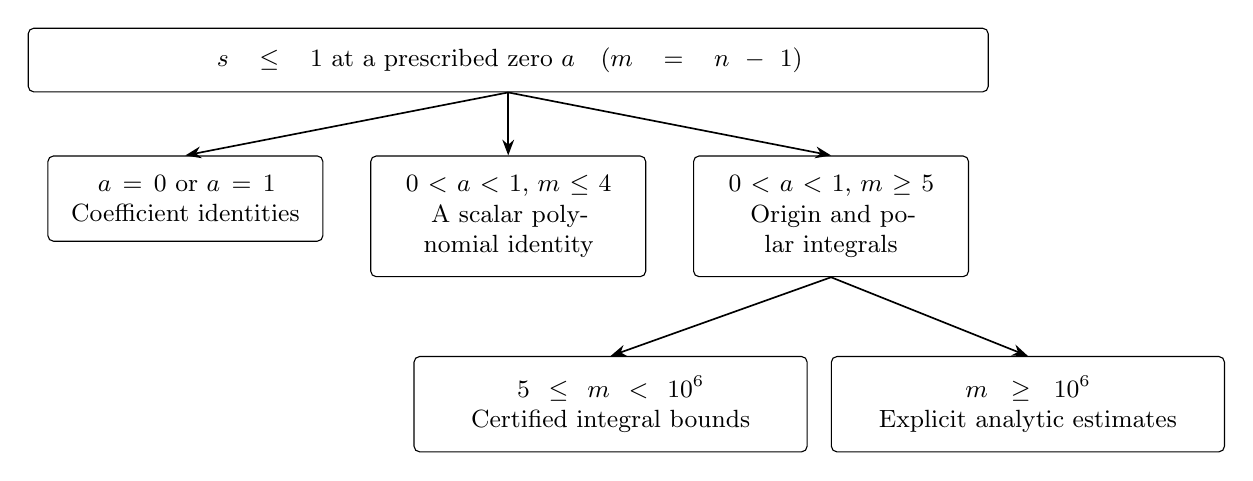
\begin{tikzpicture}[every node/.style={font=\small},
 box/.style={draw,rounded corners=2pt,align=center,inner sep=7pt},
 arr/.style={-{Stealth[length=2mm]},semithick}]
\node[box,text width=11.7cm] (top) {$s\le1$ at a prescribed zero $a$\quad ($m=n-1$)};
\node[box,text width=3.0cm,below=8mm of top,xshift=-4.1cm] (end) {$a=0$ or $a=1$\\Coefficient identities};
\node[box,text width=3.0cm,below=8mm of top] (small) {$0<a<1$, $m\le4$\\A scalar polynomial identity};
\node[box,text width=3.0cm,below=8mm of top,xshift=4.1cm] (middle) {$0<a<1$, $m\ge5$\\Origin and polar integrals};
\node[box,text width=4.5cm,below=10mm of middle,xshift=-2.8cm] (finite) {$5\le m<10^6$\\Certified integral bounds};
\node[box,text width=4.5cm,below=10mm of middle,xshift=2.5cm] (tail) {$m\ge10^6$\\Explicit analytic estimates};
\draw[arr] (top.south) -- (end.north);
\draw[arr] (top.south) -- (small.north);
\draw[arr] (top.south) -- (middle.north);
\draw[arr] (middle.south) -- (finite.north);
\draw[arr] (middle.south) -- (tail.north);
\end{tikzpicture}
\caption{The endpoint $a=1$ retains the equality cases. Every other branch excludes $s\le1$.}
\label{fig:proof}
\end{figure}

\section{Polynomial identities}\label{sec:identities}

Multiplication by a nonzero constant and rotation do not affect the desired inequality. After rotating the prescribed zero to $a\in[0,1]$ and translating by $a$, we may therefore work with
\[
 P(z)=z\prod_{i=1}^m(z-z_i),\qquad |a+z_i|\le1,\qquad m=n-1.
\]
A critical point at the origin gives an infinite summand. We may assume that this does not occur. In particular, the distinguished zero is simple, each $z_i$ is nonzero, and the translated critical points can be written as $-1/q_j$ with $q_j\ne0$.

Until Section~\ref{sec:completion}, suppose that $0<a<1$ and
\begin{equation}\label{eq:assumption}
 s=\frac1m\sum_{j=1}^m|q_j|^2\le1.
\end{equation}
We set
\[
 \mu=\frac1m\sum_jq_j=x+iy,\qquad u=|\mu|,\qquad
 \delta=1-a^2,\qquad \alpha=\frac{m\delta}{2},
\]
and define
\[
 h=2ax-a^2,\qquad \beta=1-h,\qquad
 B_s(t)=1-2axt+a^2st^2,\qquad B(t)=1-2axt+a^2t^2.
\]
In particular, $|x|\le u\le\sqrt s\le1$. Finally, let
\[
 F(t)=\prod_{j=1}^m(1-atq_j),\quad I=\int_0^1F(t)\dd t,\quad
 Z=\prod_{i=1}^m(a+z_i),\quad Q=\prod_{j=1}^m q_j,\quad J=ZQ.
\]
The disk condition and the arithmetic--geometric mean inequality imply
\begin{equation}\label{eq:Jupper}
 |J|\le |Q|\le s^{m/2}\le1.
\end{equation}
This upper bound is the part of the argument that remembers all the zeros of $P$.

The integral identities below are the translated forms of those in \cite[Section~3, pp.~3--4]{Maz26} and \cite[Lemma~6, (8)--(10)]{Tao26}. We include their derivation because it does not require a pointwise bound on the $q_j$.

\begin{lem}\label{lem:origin}
Under \eqref{eq:assumption},
\begin{equation}\label{eq:origin}
 (-1)^mJ=(m+1)I.
\end{equation}
If
\[
 R=a^2\int_0^1t\sum_{j=1}^m q_j^2
             \prod_{k\ne j}(1-atq_k)\dd t,
\]
then
\begin{equation}\label{eq:derivative}
 1=F(1)+ma\mu I+R.
\end{equation}
\end{lem}

\begin{proof}
The derivative has leading coefficient $m+1$ and zeros $-1/q_j$, so
\[
 P'(z)=\frac{m+1}{Q}\prod_j(1+zq_j).
\]
Integrating from $-a$ to $0$ and using $P(-a)=(-1)^{m+1}aZ$ proves \eqref{eq:origin}. To obtain \eqref{eq:derivative}, differentiate the product defining $F$. The identity
\[
 \prod_{k\ne j}(1-atq_k)=F(t)+atq_j\prod_{k\ne j}(1-atq_k)
\]
gives
\[
 F'(t)=-ma\mu F(t)-a^2t\sum_jq_j^2\prod_{k\ne j}(1-atq_k).
\]
Integrating over $[0,1]$ proves the assertion.
\end{proof}

A simple bound for a product with one factor omitted will be used twice. For $m\ge2$, nonnegative numbers $b_1,\ldots,b_m$, and $r=(m-1)/2$, the arithmetic--geometric mean inequality gives
\begin{equation}\label{eq:deleted}
 \prod_{k\ne j}b_k
 \le\left(\frac{\sum_kb_k^2}{m-1}\right)^r
 \le\gamma\left(\frac1m\sum_kb_k^2\right)^r,
 \qquad \gamma:=\frac53.
\end{equation}
Here $(m/(m-1))^r\le\sqrt{\e}<5/3$. In particular, the remainder in Lemma~\ref{lem:origin} satisfies the following estimates.

\begin{lem}\label{lem:rawerrors}
For $m\ge2$ and $r=(m-1)/2$,
\begin{equation}\label{eq:rawerrors}
 |F(1)|\le B_s(1)^{m/2},\qquad
 |R|\le\gamma a^2m\int_0^1tB_s(t)^r\dd t.
\end{equation}
\end{lem}

\begin{proof}
The mean of $|1-atq_j|^2$ is $B_s(t)$. Apply the arithmetic--geometric mean inequality to $F(1)$ and \eqref{eq:deleted} to each product in $R$, and use $\sum_j|q_j|^2=ms\le m$.
\end{proof}

\section{Polar estimates}\label{sec:polar}

The origin identity has an upper bound supplied by the disk. An integral in the opposite direction has a lower bound supplied by the same disk. This is the polar identity in \cite[Lemma~6, (8)]{Tao26}; its scalar consequences are developed there in Proposition~10. We use a weaker rational estimate than the one in that proposition, together with a sharper endpoint estimate from the unsimplified integral.

\begin{lem}\label{lem:polar}
Under \eqref{eq:assumption},
\begin{equation}\label{eq:polarraw}
 1\le\int_0^1\bigl(a^2+2a\delta xt+\delta^2st^2\bigr)^{m/2}\dd t.
\end{equation}
\end{lem}

\begin{proof}
Integrating the factorization of $P'$ from $0$ to $\delta/a$ and comparing with the zero factorization of $P$ gives
\[
 \int_0^1\prod_j(a+\delta tq_j)\dd t
 =\prod_i\frac{1-a(a+z_i)}{a-(a+z_i)}.
\]
The denominators are nonzero because $z_i\ne0$. For $|w|\le1$,
\[
 |1-aw|^2-|a-w|^2=\delta(1-|w|^2)\ge0.
\]
The product on the right therefore has modulus at least one. Apply the triangle inequality and then the arithmetic--geometric mean inequality to the squared moduli of the factors on the left. Their mean is the quadratic in \eqref{eq:polarraw}.
\end{proof}

We next record the restrictions on the real part of the mean that will be needed throughout the proof. The strict inequalities remain valid when $s=1$.

\begin{lem}\label{lem:h}
Under \eqref{eq:assumption},
\begin{equation}\label{eq:hbound}
 0<h<1,\qquad x>\frac a2,\qquad
 h>\frac1{1+\alpha}.
\end{equation}
For $\alpha\ge1$, one also has
\begin{equation}\label{eq:hlog}
 h>\frac{\log\alpha}{\alpha}.
\end{equation}
\end{lem}

\begin{proof}
For $0<t<1$, the use of $t^2<t$ makes the exponential majorization of \eqref{eq:polarraw} strict, even under the non-strict assumption $s\le1$. Thus
\begin{equation}\label{eq:exppolar}
 1<\int_0^1\exp\{\alpha[-1+(1+h)t]\}\dd t.
\end{equation}
If $h\le0$, the integral is less than one. Hence $h>0$, which also gives $x>a/2$. Since $x\le1$ and $a<1$, we have $h\le2a-a^2<1$. Evaluation of \eqref{eq:exppolar} now gives
\[
 \e^{\alpha h}-\e^{-\alpha}>\alpha(1+h).
\]
In particular, $\e^{\alpha h}>\alpha$, proving \eqref{eq:hlog}.

For the rational estimate, put $z=\alpha/(1+\alpha)$. Integration of the derivative of $\log(1+\alpha)-\alpha/(1+\alpha)$ shows that $z<\log(1+\alpha)$. Consequently,
\[
 \e^z-1-z<\frac{z^2\e^z}{2}
       <\frac{\alpha^2}{2(1+\alpha)}.
\]
On the other hand,
\[
 \alpha-1+\e^{-\alpha}
 =\int_0^\alpha(1-\e^{-t})\dd t
 >\int_0^\alpha\frac{t}{1+\alpha}\dd t
 =\frac{\alpha^2}{2(1+\alpha)}.
\]
If $\alpha h\le z$, monotonicity of $\e^w-1-w$ for $w\ge0$ would yield
$\e^{\alpha h}-\e^{-\alpha}<\alpha+\alpha h$, a contradiction. This proves the remaining part of \eqref{eq:hbound}.
\end{proof}

The following estimate retains more information at the far endpoint of the polar integral. It will be used both in the large-degree proof and in validating the finite certificate.

\begin{lem}\label{lem:gap}
Let
\[
 \rho=\delta s-1+2ax=h-\delta(1-s),\qquad
 N=\frac{m+2}{2},\qquad A=N\delta.
\]
Then $0<\rho\le h$ and
\begin{equation}\label{eq:chordpolar}
 (1+\delta\rho)^N-a^{2N}-N\delta(1+\rho)\ge0.
\end{equation}
For $A>1$,
\begin{equation}\label{eq:rhobounds}
 \rho\ge\frac{\log A}{A},\qquad
 B_s(1)\le1-\rho,\qquad x^2\ge\rho.
\end{equation}
\end{lem}

\begin{proof}
The quadratic $H(t)=a^2+2a\delta xt+\delta^2st^2$ is convex, with endpoint values $a^2$ and $1+\delta\rho$. It lies below the chord
\[
 \ell_\rho(t)=a^2+\delta(1+\rho)t.
\]
If $\rho\le0$, this chord is at most one and is strictly less than one on a set of positive measure. This contradicts \eqref{eq:polarraw}. Thus $\rho>0$; also $\rho\le h$ follows from $s\le1$. Integrating $\ell_\rho^{m/2}$ proves \eqref{eq:chordpolar}. In particular, $(1+\delta\rho)^N\ge A$. Taking logarithms and using $\log(1+t)\le t$ gives the first estimate in \eqref{eq:rhobounds}. The other two follow from
\[
 B_s(1)=s-\rho\le1-\rho,\qquad
 \rho\le h=x^2-(x-a)^2\le x^2.
\]
\end{proof}

\section{A centered product estimate}\label{sec:centered}

The direct estimates in Lemma~\ref{lem:rawerrors} do not use the smallness of the variance. To retain it, write
\[
 \xi_j=q_j-\mu,\qquad
 v=\frac1m\sum_j|\xi_j|^2=s-u^2\le1-u^2,
 \qquad \sum_j\xi_j=0.
\]
Instead of expanding into elementary symmetric functions, interpolate between the constant configuration $q_j=\mu$ and the given configuration.

\begin{lem}\label{lem:centered}
For $m\ge2$, $r=(m-1)/2$, and $D(t)=1-at\mu$,
\begin{equation}\label{eq:centered}
 |F(t)-D(t)^m|
 \le\frac{\gamma ma^2t^2v}{2|D(t)|}\,B_s(t)^r
 \qquad(0\le t\le1).
\end{equation}
\end{lem}

\begin{proof}
Set
\[
 G_\theta(t)=\prod_j\bigl(D(t)-at\theta\xi_j\bigr),
 \qquad 0\le\theta\le1.
\]
The cancellation $\sum_j\xi_j=0$ gives the exact identity
\begin{equation}\label{eq:interpolation}
 D(t)\,\partial_\theta G_\theta(t)
 =-a^2t^2\theta\sum_j\xi_j^2
          \prod_{k\ne j}\bigl(D(t)-at\theta\xi_k\bigr).
\end{equation}
Indeed, replace $D(t)$ in the $j$th summand of $D(t)\partial_\theta G_\theta(t)$ by
$D(t)-at\theta\xi_j+at\theta\xi_j$; the terms containing $G_\theta$ sum to zero.
Moreover,
\[
 \frac1m\sum_j|\mu+\theta\xi_j|^2=u^2+\theta^2v\le s,
 \qquad \frac1m\sum_j(\mu+\theta\xi_j)=\mu.
\]
The mean square of $D(t)-at\theta\xi_j$ is therefore at most $B_s(t)$. Apply \eqref{eq:deleted} in \eqref{eq:interpolation} and use $\sum_j|\xi_j^2|=mv$. Since $|at\mu|<1$, division by $D(t)$ is legitimate. Integrating in $\theta$ gives \eqref{eq:centered}.
\end{proof}

We now express the contradiction in terms of scalar integrals. Define
\begin{equation}\label{eq:Cdef}
 C(a,x,m)=\frac{\gamma a^3m(m+1)}2
      \int_0^1\frac{t^2B(t)^{(m-1)/2}}{1-axt}\dd t.
\end{equation}
The denominator is positive because $ax<1$.

\begin{prop}\label{prop:scalar}
Under \eqref{eq:assumption}, for $m\ge2$ one has
\begin{equation}\label{eq:centerscalar}
 1\le au+C(a,x,m)u(1-u^2)+\beta^{(m+1)/2}
\end{equation}
and
\begin{equation}\label{eq:directscalar}
 1\le\beta^{m/2}+\frac{ma}{m+1}
       +\gamma a^2m\int_0^1tB(t)^{(m-1)/2}\dd t.
\end{equation}
\end{prop}

\begin{proof}
By \eqref{eq:hbound}, $\mu\ne0$. Direct integration gives
\[
 (m+1)\int_0^1D(t)^m\dd t
 =\frac{1-D(1)^{m+1}}{a\mu}.
\]
Multiply the integrated estimate \eqref{eq:centered} by $a|\mu|(m+1)$. Using $B_s\le B$, $|D(t)|\ge1-axt$, and \eqref{eq:Cdef}, we obtain
\[
 \left|a\mu(m+1)I-\bigl(1-D(1)^{m+1}\bigr)\right|
 \le C(a,x,m)uv.
\]
Also $|D(1)|^2\le B(1)=\beta$. Now apply \eqref{eq:origin}, \eqref{eq:Jupper}, and $v\le1-u^2$ to get \eqref{eq:centerscalar}. Finally, \eqref{eq:derivative}, \eqref{eq:rawerrors}, $u\le1$, and $|I|\le1/(m+1)$ give \eqref{eq:directscalar}.
\end{proof}

The optimization over $u$ involves only a cubic. For $a,C\ge0$, put
\begin{equation}\label{eq:cubicmax}
 \M(a,C)=\max_{0\le u\le1}\{au+Cu(1-u^2)\}
 =\begin{cases}
 a,&2C\le a,\\[1mm]
 \displaystyle\frac{2(a+C)^{3/2}}{3\sqrt{3C}},&2C>a.
 \end{cases}
\end{equation}
This follows by differentiating $(a+C)u-Cu^3$. The function $\M$ is nondecreasing in each of its arguments, directly from its definition as a maximum. Thus an upper bound less than one for either right-hand side in Proposition~\ref{prop:scalar} is enough; no information about the argument of $\mu$ is needed.

\section{Large degrees}\label{sec:large}

We first dispose of the infinite range of degrees. The threshold used here is chosen to leave generous margins in the elementary estimates; its precise value has no significance for the final theorem. Set
\[
 M_0=10^6.
\]
All comparisons in this section are uniform for $m\ge M_0$. Appendix~\ref{app:constants} gives rational checks at the endpoint and the monotonicity facts used to extend them.

\subsection{Zeros near the unit circle}
In this range the centered estimate is sufficient on its own.

\begin{prop}\label{prop:near}
Assumption \eqref{eq:assumption} is impossible when $m\ge M_0$ and $0<\delta\le1/10$.
\end{prop}

\begin{proof}
We have $a^2\ge9/10$, $a\ge9/10$, and $\alpha\le m/20$. Write
$r=(m-1)/2$ and $\nu=(m-3)/2$. We first claim that
\begin{equation}\label{eq:tailpowers}
 \beta^\nu\le m^{-4},\qquad
 (133/160)^\nu\le m^{-4}.
\end{equation}
If $\alpha\le\sqrt m$, then \eqref{eq:hbound} and $\nu\ge m/3$ give
\[
 \nu h>\frac{m/3}{1+\sqrt m}\ge\frac{\sqrt m}{6}>4\log m.
\]
If $\sqrt m\le\alpha\le m/20$, then $\nu/\alpha\ge9$; hence \eqref{eq:hlog} gives
$\beta^\nu\le\exp(-\nu h)<\alpha^{-9}\le m^{-9/2}$.
This proves the first part of \eqref{eq:tailpowers}. The second follows from
\[
 (133/160)^\nu\le\exp(-27\nu/160)
 \le\exp(-9m/160)\le m^{-4}.
\]

We estimate \eqref{eq:Cdef} by splitting its integral at $t=1/4$. For $0\le t\le1/4$, the inequality $x>a/2$ gives
\[
 B(t)\le1-\frac{3a^2t}{4}\le\exp(-3a^2t/4),
 \qquad 1-axt\ge\frac34.
\]
Using $\int_0^\infty t^2\e^{-kt}\dd t=2/k^3$, the contribution of this interval to $C$ is at most
\[
 \frac{2048\gamma m(m+1)}{81(m-1)^3a^3}<\frac{60}{m}.
\]
On $[1/4,1]$, convexity gives
\[
 B(t)\le\max\{B(1/4),B(1)\}
       \le\max\{133/160,\beta\}.
\]
Furthermore, $B(t)\le2(1-axt)$, since $a^2t^2\le1$. By \eqref{eq:tailpowers}, the remaining contribution to $C$ is at most
\[
 \gamma a^3m(m+1)\bigl\{(133/160)^\nu+\beta^\nu\bigr\}
 <\frac7{m^2}.
\]
It follows that
\begin{equation}\label{eq:Cnear}
 C<\frac{61}{m}<\frac a2.
\end{equation}

It remains to keep the endpoint error on the scale of $\delta$. Set $E=\beta^{(m+1)/2}$. If $\alpha\ge1$, then \eqref{eq:tailpowers} and $\delta=2\alpha/m$ imply
$E/\delta\le1/(2m^3)<1/4$. If $0<\alpha\le1$, then \eqref{eq:hbound} gives $\beta\le\min\{\alpha,1/2\}$, so
\[
 \frac E\delta\le m2^{-(m+1)/2}<\frac14.
\]
Combining this estimate with \eqref{eq:Cnear} and \eqref{eq:cubicmax}, the right-hand side of \eqref{eq:centerscalar} is less than
\[
 a+\frac{1-a^2}{4}<1.
\]
This is the required contradiction.
\end{proof}

\subsection{The complementary range}
Away from the unit circle, the simpler derivative identity suffices. The endpoint information in Lemma~\ref{lem:gap} prevents the increasing part of the integral from contributing too much.

\begin{prop}\label{prop:away}
Assumption \eqref{eq:assumption} is impossible when $m\ge M_0$ and $\delta\ge1/10$.
\end{prop}

\begin{proof}
Use $N,A,\rho$ from Lemma~\ref{lem:gap}, so $A\ge m/20>1$. Equations \eqref{eq:rawerrors} and \eqref{eq:rhobounds} imply
\begin{equation}\label{eq:Flarge}
 |F(1)|\le\exp(-m\rho/2)
       \le A^{-m/((m+2)\delta)}.
\end{equation}
Let $r=(m-1)/2$ and $t_0=x/(as)$. Here $s>0$ because the $q_j$ are nonzero. Split the integral defining $R$ at $\min\{1,t_0\}$ and denote the two contributions by $R_{\rm dec}$ and $R_{\rm inc}$; the second is zero when $t_0\ge1$.
On the decreasing part, $B_s(t)\le1-axt\le\e^{-axt}$. Therefore
\begin{equation}\label{eq:Rdec}
 |R_{\rm dec}|
 \le\frac{\gamma a^2m}{(rax)^2}
 =\frac{4\gamma m}{(m-1)^2x^2}<\frac7{mx^2}.
\end{equation}
On the increasing part, $B_s(t)\le B_s(1)\le1-\rho$. With $\sigma=(m-1)/(m+2)$, we obtain
\begin{equation}\label{eq:Rinc}
 |R_{\rm inc}|\le\gamma a^2m A^{-\sigma/\delta}.
\end{equation}
We will prove $|F(1)|+|R|<1-a$.

Suppose first that $0<a\le1/2$. Then $\delta\ge3/4$ and $A\ge3m/8$. The estimate $x^2\ge\rho\ge\log A/A$ from \eqref{eq:rhobounds} gives
\[
 |R_{\rm dec}|<\frac{7N\delta}{m\log A}<0.292.
\]
Write $\varepsilon=a^2$ and $\eta=3/(m+2)$, so $\sigma=1-\eta$ and $\delta=1-\varepsilon$. We have
\[
 (2/\delta)^{\sigma/\delta}\le(8/3)^{4/3}<4,
 \qquad m^{\eta/\delta}\le m^{4/(m+2)}<1.001.
\]
Since $m^{1-\sigma/\delta}=m^{(\eta-\varepsilon)/\delta}
\le m^{\eta/\delta}m^{-\varepsilon}$, \eqref{eq:Rinc} yields
\[
 |R_{\rm inc}|<4\gamma(1.001)\varepsilon m^{-\varepsilon}
 \le\frac{4\gamma(1.001)}{\e\log m}
 <\frac5{2\log m}<\frac5{26}.
\]
Here the maximum of $\varepsilon\e^{-\varepsilon\log m}$ on $[0,\infty)$ is $1/(\e\log m)$. Also \eqref{eq:Flarge} gives $|F(1)|<10^{-4}$, since $A>10^5$ and $m/((m+2)\delta)>4/5$. Thus
\[
 |F(1)|+|R|<0.292+\frac5{26}+10^{-4}<\frac12\le1-a.
\]

Now suppose that $a\ge1/2$. Then $1/10\le\delta\le3/4$ and $x>a/2\ge1/4$, so \eqref{eq:Rdec} gives $|R_{\rm dec}|<112/m$. The function
\[
 g(\delta)=(1-\delta)(m\delta/2)^{-\sigma/\delta}
\]
is increasing on $[1/10,3/4]$. Indeed,
\[
 \frac{g'(\delta)}{g(\delta)}
 =-\frac1{1-\delta}
   +\frac{\sigma}{\delta^2}\{\log(m\delta/2)-1\}
 >-4+\frac9{10}\frac{16}{9}\,3>0.
\]
Using $A\ge m\delta/2$ in \eqref{eq:Rinc}, and retaining the relation $a^2=1-\delta$, we find
\begin{equation}\label{eq:Rincsmall}
 |R_{\rm inc}|\le\frac5{12}m(3m/8)^{-4\sigma/3}<0.016.
\end{equation}
For completeness, $4\sigma/3>33333/25000=4/3-1/75000$, and the function
$m(3m/8)^{-33333/25000}$ decreases for $m\ge M_0$. At $m=M_0$, the inequalities
\[
 72^3<375000,\qquad 375000^{1/75000}<1.001
\]
bound it by $1.001/27$, proving the last comparison in \eqref{eq:Rincsmall}.

Similarly, with $k=m/(m+2)$ the function $(m\delta/2)^{-k/\delta}$ is increasing in $\delta$, because its logarithmic derivative is
$k\{\log(m\delta/2)-1\}/\delta^2>0$. Equation \eqref{eq:Flarge} therefore gives
\[
 |F(1)|\le(3m/8)^{-4k/3}<\frac8{3m}.
\]
Altogether,
\[
 |F(1)|+|R|<\frac{112}{m}+\frac8{3m}+0.016
 <0.017<\frac1{20}<1-\sqrt{9/10}\le1-a.
\]

In both cases, \eqref{eq:origin} and \eqref{eq:derivative} now imply
\[
 |J|=\frac{m+1}{ma u}|1-F(1)-R|
 \ge\frac{m+1}{ma u}\bigl(1-|F(1)|-|R|\bigr)
 >\frac{m+1}{m u}>1,
\]
contrary to \eqref{eq:Jupper}.
\end{proof}

\section{Finite verification}\label{sec:finite}

It remains to exclude $5\le m<M_0$. This section reduces that assertion to a finite collection of rational comparisons. The certificate is a covering of a continuous parameter region, not a list of sample points. The inequalities to be checked are consequences of Proposition~\ref{prop:scalar}, and every integral is bounded from above by convexity.

\subsection{Bounds on a parameter rectangle}
Fix integers $5\le m_-\le m_+$ and real numbers $0\le a_-<a_+\le1$. Consider
\begin{equation}\label{eq:box}
 m_-\le m\le m_+,\qquad a_-\le a\le a_+,
 \qquad 0<a<1.
\end{equation}
Set $\delta_-=1-a_+^2$ and $\delta_+=1-a_-^2$. The next lemma explains the two tests used to obtain a common lower bound for $h$.

\begin{lem}\label{lem:boxpolar}
Let $h_0\in[0,1)$. Every configuration satisfying \eqref{eq:assumption} and \eqref{eq:box} has $h>h_0$ if either
\begin{equation}\label{eq:boxrational}
 h_0\le\frac1{1+m_+\delta_+/2}
\end{equation}
or
\begin{equation}\label{eq:boxchord}
 (1+\delta_+h_0)^{(m_++2)/2}
 -a_-^{m_++2}-\frac{m_-+2}{2}\delta_-(1+h_0)<0.
\end{equation}
\end{lem}

\begin{proof}
Condition \eqref{eq:boxrational} follows immediately from \eqref{eq:hbound}. To prove the other assertion, fix the actual values of $m,a$ and put
\[
 \Phi(r)=(1+\delta r)^{(m+2)/2}
       -a^{m+2}-\frac{m+2}{2}\delta(1+r).
\]
The left side of \eqref{eq:boxchord} bounds $\Phi(h_0)$ from above. Hence $\Phi(h_0)<0$. Equivalently,
\[
 \int_0^1\bigl(a^2+\delta(1+h_0)t\bigr)^{m/2}\dd t<1.
\]
The integral in this display is strictly increasing as a function of $h_0\ge0$. By \eqref{eq:chordpolar}, its value with $h_0$ replaced by $\rho$ is at least one. Thus $\rho>h_0$, and $h\ge\rho>h_0$. Notice that the monotone function used here is the chord integral; no monotonicity assertion about $\Phi$ is needed.
\end{proof}

Choose such an $h_0$, and set
\[
 d=\frac{a_+^2+h_0}{2},\qquad r_- =\frac{m_--1}{2},\qquad
 b(t)=1-h_0t-a_-^2t(1-t).
\]
We require $d<1$, as is verified for every rectangle in the certificate. Define
\begin{equation}\label{eq:Kdef}
 K_1=\int_0^1t b(t)^{r_-}\dd t,\qquad
 K_2=\int_0^1\frac{t^2b(t)^{r_-}}{1-dt}\dd t.
\end{equation}
These integrals are well defined on every rectangle, not just on feasible ones. Indeed,
\[
 b(t)=(1-t)^2+(1-h_0)t+(1-a_-^2)t(1-t)>0,
 \qquad 0\le t\le1,
\]
and $b(t)\le1$. On a feasible configuration one also has $b(t)\ge B(t)$.

\begin{lem}\label{lem:boxbounds}
On every feasible rectangle \eqref{eq:box}, the quantities
\[
 \begin{aligned}
 \overline F&=(1-h_0)^{m_-/2},&
 \overline R&=\gamma a_+^2m_+K_1,\\
 \overline E&=(1-h_0)^{(m_-+1)/2},&
 \overline C&=\frac{\gamma a_+^3m_+(m_++1)}2K_2
 \end{aligned}
\]
are upper bounds for, respectively, $\beta^{m/2}$,
$\gamma a^2m\int_0^1tB(t)^{(m-1)/2}\dd t$,
$\beta^{(m+1)/2}$, and $C(a,x,m)$.
\end{lem}

\begin{proof}
For fixed $a$ and $r=(m-1)/2\ge1$, write
\[
 B_h(t)=1-ht-a^2t(1-t),\qquad D_h(t)=1-(a^2+h)t/2.
\]
Along the interval from $h_0$ to the actual $h$, these functions are positive, and $B_h(t)\le2D_h(t)$. Hence
\[
 \frac{\partial}{\partial h}\log\frac{B_h(t)^r}{D_h(t)}
 =-\frac{rt}{B_h(t)}+\frac{t}{2D_h(t)}\le0.
\]
After replacing $h$ by $h_0$, use $a_-^2$ in the numerator and $a_+^2$ in the denominator. The resulting numerator is $b(t)$ on a feasible configuration, and $0\le b(t)\le1$. Replacing $r$ by the smaller exponent $r_-$ therefore only enlarges the bound. This proves the assertion for $\overline C$. The same argument without the denominator proves the one for $\overline R$. The endpoint estimates follow from $h>h_0$ and the lower bound on $m$.
\end{proof}

The next proposition states all four tests used by the certificate. Each test is an inequality with a strict margin, including those for rectangles that reach $a=1$.

\begin{prop}\label{prop:boxtests}
A rectangle \eqref{eq:box} contains no configuration satisfying \eqref{eq:assumption} if any one of the following four conditions holds:
\begin{align}
 &\overline F+\overline R+\frac{m_+a_+}{m_++1}<1;
 \label{eq:testdirect}\\
 &2\overline C\le a_+,\qquad a_++\overline E<1;
 \label{eq:testmonotone}\\
 &2\overline C>a_+,\quad\overline E<1,\quad
 4(a_++\overline C)^3<27\overline C(1-\overline E)^2;
 \label{eq:testcubic}\\
 &2\overline C\le a_-,\quad 0<A_+\le\tau_--1,\quad
 \frac{m_+}{2A_+}\left(\frac{A_+}{1+A_+}\right)^{\tau_-}<\frac14,
 \label{eq:testboundary}
\end{align}
where $A_+=m_+\delta_+/2$ and $\tau_-=(m_-+1)/2$.
\end{prop}

\begin{proof}
Condition \eqref{eq:testdirect} contradicts \eqref{eq:directscalar} by Lemma~\ref{lem:boxbounds}. Conditions \eqref{eq:testmonotone} and \eqref{eq:testcubic} each imply
$\M(a_+,\overline C)+\overline E<1$ by \eqref{eq:cubicmax}. Monotonicity of $\M$ in its two arguments then contradicts \eqref{eq:centerscalar}. It is not necessary that the actual $C$ and $a$ lie in the same branch of \eqref{eq:cubicmax} as $\overline C$ and $a_+$.

For \eqref{eq:testboundary}, the bound $C\le a/2$ holds throughout the rectangle. By \eqref{eq:hbound},
\[
 \frac{\beta^{(m+1)/2}}{\delta}
 \le\frac{m_+}{2}\frac{\alpha^{\tau_--1}}{(1+\alpha)^{\tau_-}}.
\]
The expression $\alpha^{\tau_--1}/(1+\alpha)^{\tau_-}$ increases for $0<\alpha\le\tau_--1$: its logarithmic derivative has the sign of $\tau_--1-\alpha$. Since $\alpha\le A_+$, condition \eqref{eq:testboundary} gives $\beta^{(m+1)/2}<\delta/4$. Equations \eqref{eq:cubicmax} and \eqref{eq:centerscalar} now contradict $a+\delta/4<1$.
\end{proof}

\subsection{Rigorous integration}
The remaining issue is to bound the integrals in \eqref{eq:Kdef}. We use only convexity. In particular, no error estimate for a floating-point quadrature rule is assumed.

\begin{lem}\label{lem:quadrature}
The functions $b(t)^{r_-}$ and $b(t)^{r_-}/(1-dt)$ are convex on $[0,1]$. For any convex function $f$ on $[l,l+z]$, with $z>0$ and $l\ge0$,
\begin{equation}\label{eq:weights}
 \begin{aligned}
 \int_l^{l+z}tf(t)\dd t
 &\le z\left(\frac l2+\frac z6\right)f(l)
      +z\left(\frac l2+\frac z3\right)f(l+z),\\
 \int_l^{l+z}t^2f(t)\dd t
 &\le z\left(\frac{l^2}2+\frac{lz}3+\frac{z^2}{12}\right)f(l)\\
 &\quad+z\left(\frac{l^2}2+\frac{2lz}3+\frac{z^2}4\right)f(l+z).
 \end{aligned}
\end{equation}
\end{lem}

\begin{proof}
The function $b$ is a nonnegative convex quadratic. Since $r_-\ge2$, $b^{r_-}$ is convex. For $q\ge2$, the function $(B,D)\mapsto B^q/D$ is convex on $B\ge0,D>0$ and is nondecreasing in $B$. For $B>0$ this follows from the nonnegative diagonal entries of its Hessian and the determinant
\[
 q(q-2)B^{2q-2}/D^4\ge0;
\]
the boundary $B=0$ follows by continuity. Composing with the convex function $b(t)$ and the positive affine function $1-dt$ proves the second convexity assertion. Finally, a convex function is bounded above by its endpoint chord. Multiplying that chord by $t$ or $t^2$ and integrating gives \eqref{eq:weights}.
\end{proof}

\subsection{The certificate and its verification}
Let $S=2^{100}$. A certificate record has the form
\[
 (m_-,m_+,L_a,U_a,H_0,\text{test},v_0),
\]
where $L_a,U_a,H_0$ are integers encoding
$a_-=L_a/S$, $a_+=U_a/S$, and $h_0=H_0/S$, and $v_0$ is a positive integer controlling the integration mesh. Appendix~\ref{app:format} gives the corresponding positional schema in the supplied JSON file.

For a given $m_+$, let $K=\lfloor\log_2m_+\rfloor+4$. Start with the integer breakpoints
\[
 0,\ S\mathbin{\gg}K,\ S\mathbin{\gg}(K-1),\ldots,
 S\mathbin{\gg}1,\ S,
\]
where $S\mathbin{\gg}k=\lfloor S/2^k\rfloor$. In each consecutive interval $[L,U]$, insert $L+\lfloor j(U-L)/v_0\rfloor$ for $0\le j\le v_0$, add all reflected points $S-t$, sort, and divide by $S$. All vertices and all weights in \eqref{eq:weights} are thus rational. The original checker encloses each arithmetic operation on a $100$-bit dyadic grid. The second checker computes coordinates, weights, and rational coefficients exactly, and encloses powers on a $160$-bit dyadic grid. Nonintegral exponents are only half-integers, so they require integer powers and square-root enclosures, not transcendental evaluation.

The finite computational assertion needed for the proof is as follows.

\begin{prop}\label{prop:finite}
For every integer $5\le m<10^6$ and every $0<a<1$, assumption \eqref{eq:assumption} is impossible.
\end{prop}

\begin{proof}
The file \code{certificate.json} in the supplementary material contains $6593$ records in $430$ consecutive degree blocks. For each record, both verification programs check the range of its endpoints, one of \eqref{eq:boxrational} and \eqref{eq:boxchord}, the positivity of $1-d$, the integral bounds from \eqref{eq:weights}, and one of the four inequalities in Proposition~\ref{prop:boxtests}. The accepted records are distributed as follows:
\begin{center}
\begin{tabular}{lr}
\toprule
Exclusion condition & Number of records\\
\midrule
\eqref{eq:testdirect} & 4003\\
\eqref{eq:testmonotone} & 5\\
\eqref{eq:testcubic} & 2054\\
\eqref{eq:testboundary} & 531\\
\midrule
Total & 6593\\
\bottomrule
\end{tabular}
\end{center}
Of the polar bounds, $513$ use \eqref{eq:boxrational} and $6080$ use \eqref{eq:boxchord}. The programs also sort the degree blocks and the intervals within each block, and verify exact endpoint adjacency: the degree range is $5,\ldots,999999$, and the intervals in $a$ cover $[0,1]$ in every block without gaps or overlaps. Every feasible pair is therefore excluded by Proposition~\ref{prop:boxtests}.

Both programs return \code{PASS} on the supplied certificate. This finite verification, with the directed-rounding rules in Appendix~\ref{app:format}, is the computational part of the proof. The certificate is identified by the SHA--256 digest
\begin{center}\small\ttfamily
8384d62a377b4fcac4080d0e05979d7a6fcf\\
90437b7e4911927a5403d4052709.
\end{center}
The line break and final punctuation are not part of the digest.
\end{proof}

\section{Completion and equality}\label{sec:completion}

The arguments above cover every interior zero once $m\ge5$. Small degrees can be handled without any certificate. The polar approach to these degrees already occurs in \cite[Section~8, pp.~16--17]{Maz26} and \cite[Section~4, Remark~16]{Tao26}. The following factorization makes the needed scalar estimate explicit.

\begin{lem}\label{lem:small}
Assumption \eqref{eq:assumption} is impossible when $1\le m\le4$ and $0<a<1$.
\end{lem}

\begin{proof}
Since $x\le1$ and $s\le1$, the integrand in \eqref{eq:polarraw} is at most $(a+\delta t)^m$. Direct integration and expansion give
\[
 1-\int_0^1\bigl(a+(1-a^2)t\bigr)^4\dd t
 =\frac{(1-a)^3(1+a)}5\bigl(a^4-3a^3+3a+4\bigr)>0.
\]
The final factor is $a^4+3a(1-a^2)+4>0$. The monotonicity of integral power means on a measure space of total mass one yields, for $m\le4$,
\[
 \int_0^1(a+\delta t)^m\dd t
 \le\left(\int_0^1(a+\delta t)^4\dd t\right)^{m/4}<1.
\]
This contradicts \eqref{eq:polarraw}.
\end{proof}

We finish with the two endpoints. The boundary identity used below is the case $k=\nu=1$ of Meir and Sharma's reciprocal identity \cite[p.~461, (3.2)]{MS69}; see also \cite[p.~26, (5.1) and Remark~5.1]{TZ25}. Its origin should be distinguished from the centered estimate of Section~\ref{sec:centered}.

\begin{lem}\label{lem:endpoints}
Suppose that none of the translated critical points is zero. At the distinguished zero $a=0$,
\[
 s\ge(m+1)^{2/m}>1.
\]
At the distinguished zero $a=1$, one has $s\ge1$, with equality precisely for nonzero constant multiples of $z^{m+1}-1$ in the original coordinate.
\end{lem}

\begin{proof}
At $a=0$, comparison of constant terms gives
\[
 \frac{m+1}{Q}=P'(0)=\prod_i(-z_i).
\]
Since $|z_i|\le1$, we obtain $|Q|\ge m+1$. The arithmetic--geometric mean inequality then gives $s\ge|Q|^{2/m}\ge(m+1)^{2/m}$.

At $a=1$, work in the original coordinate. Denote the other zeros by $\zeta_i$ and the critical points by $c_j$. The zero $1$ is simple by hypothesis. Logarithmic differentiation at $1$ gives
\[
 \sum_j\frac1{1-c_j}
 =\frac{p''(1)}{p'(1)}
 =2\sum_i\frac1{1-\zeta_i}.
\]
In fact, the following nonnegative decomposition is useful:
\begin{equation}\label{eq:boundarydefect}
 \sum_j\frac1{|1-c_j|^2}-m
 =\sum_j\frac{|c_j|^2}{|1-c_j|^2}
   +2\sum_i\frac{1-|\zeta_i|^2}{|1-\zeta_i|^2}.
\end{equation}
To verify it, put $q_j=(1-c_j)^{-1}$, use
$|q_j|^2-1=|q_j-1|^2+2\Ree q_j-2$, and substitute the reciprocal identity and
$2\Ree(1-\zeta_i)^{-1}=1+(1-|\zeta_i|^2)/|1-\zeta_i|^2$.
Every term on the right of \eqref{eq:boundarydefect} is nonnegative. Equality forces $c_j=0$ for all $j$. Thus $p'$ is a constant multiple of $z^m$, and $p(1)=0$ implies that $p$ is a nonzero constant multiple of $z^{m+1}-1$. Conversely, that polynomial has $s=1$.
\end{proof}

We can now assemble the proof of Theorem~\ref{thm:main}.

\begin{proof}
If a prescribed zero is also a critical point, \eqref{eq:main} is strict. Otherwise perform the normalization of Section~\ref{sec:identities}. For $0<a<1$, Lemma~\ref{lem:small}, Proposition~\ref{prop:finite}, and Propositions~\ref{prop:near}--\ref{prop:away} exclude $s\le1$ in all possible degrees. Hence the sum in \eqref{eq:main} is strictly greater than $m$ at an interior zero. Lemma~\ref{lem:endpoints} treats $a=0$ and $a=1$ and identifies the boundary equality case. Undoing the rotation changes $z^n-1$ to a nonzero multiple of $z^n-\omega$ with $|\omega|=1$. Conversely, every critical point of $A(z^n-\omega)$ is zero, and every zero has modulus one, so equality holds.
\end{proof}

For clarity, we also give the short proof of Corollary~\ref{cor:powers}, including its equality assertion.

\begin{proof}
When all distances are nonzero, put $t_j=|\zeta-c_j|^{-1}$. For $\lambda\ge2$, power means and \eqref{eq:main} give
\[
 \left(\frac1m\sum_jt_j^\lambda\right)^{1/\lambda}
 \ge\left(\frac1m\sum_jt_j^2\right)^{1/2}\ge1.
\]
If the $\lambda$-sum equals $m$, then the quadratic mean must equal one, so Theorem~\ref{thm:main} identifies the polynomial. Conversely, that family gives equality for every $\lambda$. A zero distance gives an infinite sum and cannot give equality.
\end{proof}

\appendix
\section{Constants and reproducibility}\label{app:audit}

\subsection{Analytic comparisons}\label{app:constants}
This appendix supplies the constant checks used in Section~\ref{sec:large}. They are also implemented with exact fractions in \code{analytic_audit.py}. No extrapolation from a finite list of large degrees is used.

The exponential series, with its tail bounded by a geometric series, gives
\[
 \frac{27}{10}<\sum_{j=0}^5\frac1{j!}<\e
 <\sum_{j=0}^5\frac1{j!}+\frac7{4320}<\frac{11}{4}.
\]
It follows by integer powers that
\[
 13<\log M_0<14,\qquad
 \log(3M_0/8)>12,\qquad \log(M_0/20)>4.
\]
In particular, $\sqrt\e<5/3$. The two comparisons
\[
 \frac{\sqrt m}{6}>4\log m,\qquad
 \frac{9m}{160}>4\log m
\]
hold at $m=M_0$ and improve thereafter: the derivatives of the left-minus-right expressions are $(\sqrt m-48)/(12m)$ and $9/160-4/m$.

For the integral constants, both
$m^2(m+1)/(m-1)^3$ and $(m/(m-1))^2$ decrease for $m>1$. At $m=M_0$ one checks
\[
 \frac{2048\gamma}{81}\left(\frac{10}{9}\right)^3
 \frac{M_0^2(M_0+1)}{(M_0-1)^3}<60,
 \qquad
 4\gamma\left(\frac{M_0}{M_0-1}\right)^2<7.
\]
These are the constants in the near-boundary integral estimate and \eqref{eq:Rdec}. The remaining near-boundary comparisons reduce to
$10(1-3/M_0)>9$, $60/M_0+7/M_0^2<61/M_0<9/20$, and
$m2^{-(m+1)/2}<1/4$ for $m\ge16$. For the last assertion, the sequence decreases because $(m+1)/m<\sqrt2$ for $m\ge16$, and its initial value is already less than $1/4$.

The function $\log m/(m+2)$ decreases for $m\ge M_0$. Using $\e^t\le(1-t)^{-1}$ for $0\le t<1$ gives
\[
 m^{4/(m+2)}
 <\frac1{1-56/(M_0+2)}<\frac{1001}{1000}.
\]
The elementary comparisons in the small-$a$ case are
\[
 (8/3)^4<4^3,\qquad
 \frac{4(5/3)(1001/1000)}{27/10}<\frac52,
 \qquad
 \frac{7(M_0+2)}{24M_0}<\frac{292}{1000},
\]
\[
 \frac{292}{1000}+\frac5{26}+\frac1{10000}<\frac12.
\]
For the other case, $\sigma>99999/100000$ and $72^3<375000$. Also
\[
 375000^{1/75000}
 <\frac1{1-14/75000}<\frac{1001}{1000},
 \qquad
 \frac5{12}\frac1{27}\frac{1001}{1000}<\frac{16}{1000}.
\]
Finally,
\[
 \frac{112}{M_0}+\frac8{3M_0}+\frac{16}{1000}<\frac{17}{1000}<\frac1{20},
 \qquad (19/20)^2>9/10.
\]
All terminating decimals used in the proof denote exact rational numbers.

\subsection{Certificate format and directed rounding}\label{app:format}
The JSON file has fields \code{precision_bits}, \code{m_start},
\code{m_stop_exclusive}, and \code{records}, together with generation statistics. The first three values are $100$, $5$, and $1000000$. Each record is a seven-entry array:
\begin{center}\small
\code{[m_lower,m_upper,a_lower_integer,a_upper_integer,h_integer,test,subdivision]}.
\end{center}
The three coordinate integers are stored as decimal strings and divided by $2^{100}$. They are exact coordinates, not decimal approximations. Every record in the supplied certificate uses \code{subdivision = 2}. The test field is an annotation; the second checker recomputes a valid test rather than trusting that annotation. The optional preliminary test $h_0>2a_+-a_+^2$ would also exclude a rectangle by \eqref{eq:hbound}; no record of this certificate needs it.

For an interval $[L/S,U/S]$ and another nonnegative interval $[L'/S,U'/S]$, multiplication is enclosed by
\[
 \left[\frac{\lfloor LL'/S\rfloor}{S},
       \frac{\lceil UU'/S\rceil}{S}\right].
\]
For a positive denominator interval the quotient is enclosed by
\[
 \left[\frac{\lfloor LS/U'\rfloor}{S},
       \frac{\lceil US/L'\rceil}{S}\right].
\]
Square roots use the integer square root of $LS$ and the corresponding upper integer square root of $US$. Signed additions and subtractions use the appropriate endpoint order. Integer powers are computed by repeated squaring, and a half-integer power is a product of an integer power and a square root. The first checker uses these rules for all operations. The second uses exact rational arithmetic except for directed power enclosures, where it uses $S=2^{160}$. The implementation also replaces interval bounds for $b$ by their nonnegative parts. This is valid because $b\ge0$, as proved before Lemma~\ref{lem:boxbounds}; truncation cannot discard its true value. These choices affect only efficiency and the width of the enclosures; an accepted comparison has the asserted rational sign.

\subsection{Reproduction and scope of verification}\label{app:reproduce}
From the supplementary directory, the following commands require only Python's standard library:
\begin{verbatim}
python verify_certificate.py certificate.json
python verify_independent.py certificate.json
python analytic_audit.py
\end{verbatim}
The first two commands verify Proposition~\ref{prop:finite}; the third checks the endpoint comparisons in Appendix~\ref{app:constants}. The recorded outputs accompany the code. The generator can be run as
\begin{verbatim}
python certify.py --stop 1000000 --out regenerated_certificate.json
python verify_independent.py regenerated_certificate.json
\end{verbatim}
Floating-point operations in the generator only propose search brackets or report progress. They never decide whether a rectangle is accepted. The stored certificate, rather than any particular search trajectory, is the reproducible object used in the proof.

The two verification programs are separate implementations of the same mathematical specification. This reduces dependence on a shared arithmetic implementation; it is not an independent mathematical proof of the reduction, a formalization in Lean, or external peer review. The analytic arguments in Sections~\ref{sec:identities}--\ref{sec:completion} remain part of the proof and must be checked as such.

\section*{Declaration of competing interest}
The author declares no competing interests.

\section*{Data availability}
The finite certificate, its generator, two verification programs, the analytic constant checker, and the recorded verification outputs are supplied as supplementary material. The certificate is an essential component of the computer-assisted proof. No empirical data are used.

\section*{Use of generative artificial intelligence}
Generative artificial intelligence was used in developing and checking arguments, constructing the verification programs, researching references, and preparing the exposition. The verification claims made in this paper are limited to the explicitly described computations and do not imply external mathematical review or proof-assistant certification.

\section*{Acknowledgments}
Teng Zhang is supported by the China Scholarship Council, the Young Elite Scientists Sponsorship Program for PhD Students (China Association for Science and Technology), and the Fundamental Research Funds for the Central Universities at Xi'an Jiaotong University (Grant No.~xzy022024045).

\begin{thebibliography}{99}
\raggedright

\bibitem[BRS85]{BRS85}
B.~D.~Bojanov, Q.~I.~Rahman, and J.~Szynal,
\emph{On a conjecture of Sendov about the critical points of a polynomial},
Math. Z. \textbf{190} (1985), no.~2, 281--285.
\doi{10.1007/BF01160464}

\bibitem[BX99]{BX99}
J.~E.~Brown and G.~Xiang,
\emph{Proof of the Sendov conjecture for polynomials of degree at most eight},
J. Math. Anal. Appl. \textbf{232} (1999), no.~2, 272--292.
\doi{10.1006/jmaa.1999.6267}

\bibitem[Cha20]{Cha20}
T.~P.~Chalebgwa,
\emph{Sendov's conjecture: A note on a paper of D\'egot},
Anal. Math. \textbf{46} (2020), no.~3, 447--463.
\doi{10.1007/s10476-020-0050-x}
Author version: arXiv:1804.09953v1 [math.CV].

\bibitem[Chi11]{Chi11}
T.~Chijiwa,
\emph{A quantitative result on Sendov's conjecture for a zero near the unit circle},
Hiroshima Math. J. \textbf{41} (2011), no.~2, 235--273.
\doi{10.32917/hmj/1314204564}

\bibitem[Deg14]{Deg14}
J.~D\'egot,
\emph{Sendov conjecture for high degree polynomials},
Proc. Amer. Math. Soc. \textbf{142} (2014), no.~4, 1337--1349.
\doi{10.1090/S0002-9939-2014-11888-0}
Author version: arXiv:1106.4126 [math.CV].

\bibitem[Hay67]{Hay67}
W.~K.~Hayman,
\emph{Research problems in function theory},
Athlone Press, London, 1967.

\bibitem[Maz26]{Maz26}
L.~Mazur,
\emph{A computer-assisted proof of Sendov's conjecture},
preprint, August 5, 2026, 19~pp.
\url{https://www.proofatlas.ai/papers/sendov-conjecture/SENDOV_CONJECTURE_PROOF_AUGUST_5_2026.pdf}

\bibitem[MS69]{MS69}
A.~Meir and A.~Sharma,
\emph{On Ilyeff's conjecture},
Pacific J. Math. \textbf{31} (1969), no.~2, 459--467.
\doi{10.2140/pjm.1969.31.459}

\bibitem[Mil93]{Mil93}
M.~J.~Miller,
\emph{On Sendov's conjecture for roots near the unit circle},
J. Math. Anal. Appl. \textbf{175} (1993), no.~2, 632--639.
\doi{10.1006/jmaa.1993.1194}

\bibitem[Mil25]{Mil25}
M.~J.~Miller,
\emph{Seeking a quadratic refinement of Sendov's conjecture},
arXiv:2506.12951v2 [math.CV], September 8, 2025, 10~pp.
\doi{10.48550/arXiv.2506.12951}

\bibitem[PR72]{PR72}
D.~Phelps and R.~S.~Rodriguez,
\emph{Some properties of extremal polynomials for the Ilieff conjecture},
Kodai Math. Sem. Rep. \textbf{24} (1972), no.~2, 172--175.
\doi{10.2996/kmj/1138846519}

\bibitem[Rub68]{Rub68}
Z.~Rubinstein,
\emph{On a problem of Ilyeff},
Pacific J. Math. \textbf{26} (1968), no.~1, 159--161.
\doi{10.2140/pjm.1968.26.159}

\bibitem[Sen02]{Sen02}
Bl.~Sendov,
\emph{Generalization of a conjecture in the geometry of polynomials},
Serdica Math. J. \textbf{28} (2002), no.~4, 283--304.
\url{https://www.math.bas.bg/serdica/2002/2002-283-304.pdf}

\bibitem[TZ25]{TZ25}
Q.~Tang and T.~Zhang,
\emph{Sharp Schoenberg type inequalities and the de Bruin--Sharma problem},
arXiv:2508.10341v3 [math.CV], December 5, 2025, 57~pp.
\doi{10.48550/arXiv.2508.10341}

\bibitem[Tao22]{Tao22}
T.~Tao,
\emph{Sendov's conjecture for sufficiently-high-degree polynomials},
Acta Math. \textbf{229} (2022), no.~2, 347--392.
\doi{10.4310/ACTA.2022.v229.n2.a3}
Author version: arXiv:2012.04125v2 [math.CV].

\bibitem[Tao26]{Tao26}
T.~Tao,
\emph{A digestion of the proof of Sendov's conjecture},
What's New, August 12, 2026.
\url{https://terrytao.wordpress.com/2026/08/12/a-digestion-of-the-proof-of-sendovs-conjecture/}

\bibitem[VZ93]{VZ93}
V.~V\^aj\^aitu and A.~Zaharescu,
\emph{Ilyeff's conjecture on a corona},
Bull. London Math. Soc. \textbf{25} (1993), no.~1, 49--54.
\doi{10.1112/blms/25.1.49}

\end{thebibliography}
\end{document}
